    \thispagestyle{plain}
	\vspace*{\fill}
    \begin{center}
      {\Huge Apéndices}\\[0.5cm]
    \end{center}
    \vspace*{\fill}


\appendix

\chapter{Tecnologías utilizadas}
\label{chap:techs}

\makeatletter
\def\cleardoublepage{\clearpage\if@twoside \ifodd\c@page\else
  \hbox{}
  \vspace*{\fill}
  \newpage
  \if@twocolumn\hbox{}\newpage\fi\fi\fi}
\makeatother

\section{Notación ABC}
\label{sec:NotacionABC}
\torev{Última revisión realizada el 25-06-2012}

En 1993, Chris Walshaw introdujo una nueva notación musical de texto plano, junto con abc2mtex (programa que traduce la notación ABC en notación que usa MusicTeX y TeX), \cite{abcDescrip}. Como resultado se obtuvo un lenguaje para escribir partituras de música. Poco después, Michael Methfessel con abc2ps y James Allwright followed con abcMIDI, empezaron a exportar la notación ABC en diferentes formatos.

Inicialmente ABC se creó para escribir música tradicional. Gradualmente se fueron añadiendo nuevas funcionalidades expandiendo sus posibilidades, pero ante todo se ha seguido preservando la mayor ventaja de esta notación: es fácil de crear, es ligera en almacenamiento (archivos de tamaño muy pequeño) y se puede compartir y transformar fácilmente, ya que es texto plano. Además, si está bien formateada la información se puede leer tras adquirir cierta experiencia.

Hoy en día hay un gran número de aplicaciones software que son compatibles con la notación ABC. Algunos programas comerciales permiten cargar o guardar la música producida en formato ABC. También existe la posibilidad de transformar del formato ABC a formato MIDI y viceversa. La oferta de software gratuito que maneja esta notación es amplia y variada. 

Gracias a todas estas características, la notación ABC se ha adoptado como solución al problema que surge de traducir la representación interna de la música dentro del sistema a formato de audio MIDI. Para conseguirlo se transforma de la notación musical interna a notación ABC y de ésta a un archivo MIDI gracias a abc2midi, que forma parte del proyecto abcMIDI.

\color{blue}No es el propósito de ese documento realizar un tutorial exhaustivo de dicha notación, sin embargo se muestran en las Figura~\ref{fig:abcexample} y ~\ref{fig:abcexample2} dos ejemplos de lo fácil que es escribir notación musical usando este estándar.\color{black}

		\begin{figure}[!htbp]
		\centering
		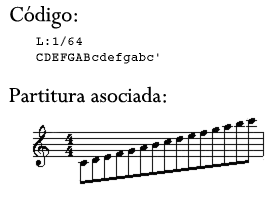
\includegraphics[scale=0.7]{graphics/abc-example.png}
		\caption{Ejemplo de notación ABC}
		\label{fig:abcexample}
		\end{figure}
		
		\begin{figure}[!htbp]
		\centering
		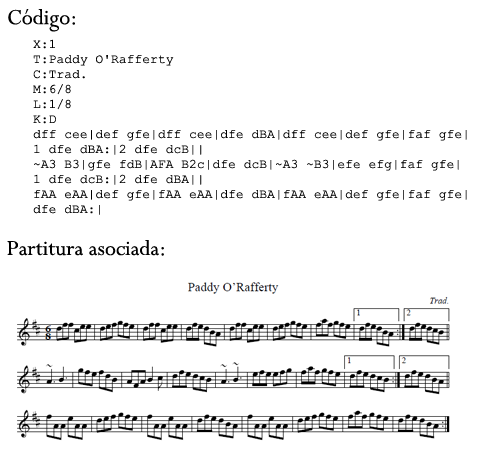
\includegraphics[scale=0.7]{graphics/abc-example2.png}
		\caption{Ejemplo de notación ABC}
		\label{fig:abcexample2}
		\end{figure}

\section{abcMIDI}
\label{sec:abcMIDI}
\gotrev{Última revisión realizada el 25-06-2012}

abcMIDI consiste un paquete de programas desarrollado por James Allwright, \cite{abcMIDIDescrip}. Su cometido principal es procesar archivos con formato notación ABC. Este paquete contiene los siguientes programas: abc2midi, abc2abc, yaps, abcm2ps y midi2abc. En el proyecto se usan tanto abc2midi (para producir archivos de audio), como abcm2ps (para producir partituras).

abc2midi sirve para convertir archivos con formato notación ABC en archivos de sonido MIDI. Es probablemente el programa más avanzado y maduro de las diferentes posibilidades de software libre disponible en la red. Además contiene funcionalidades extra como el manejo de archivos con múltiples voces, trasponer voces individuales y añadir un acompañamiento de percusión entre otros.

abcm2ps tiene como funcionalidad producir una partitura musical partiendo del archivo en notación ABC de entrada. Esta partitura puede darse en numerosos formados, siendo dos de ellos ps y xhtml. A diferencia de su versión previa, abcm2ps, permite trabajar con varias voces; aunque a día de hoy existen unas pocas características de la notación ABC que no es capaz de transformar a la correspondiente partitura.


\section{OpenCV}
\label{sec:OpenCV}
\gotrev{Última revisión realizada el 25-06-2012}

\emph{OpenCV} es una de las librerías más importantes de visión por computador en tiempo real que existen por el momento. Fue desarrollada por Intel en 1999, y desde entonces se ha extendido su uso en numerosos sectores tecnológicos, \cite{opencvDoc}.\\

Es una librería multiplataforma que ofrece funcionalidad para todo tipo de análisis y reconocimiento de imagenes, razón por la cual se ha elegido como base para la implementación del módulo de análisis de imágenes del proyecto.



\section{TiMidity}
\label{sec:Timidity}
\gotrev{Última revisión realizada el 25-06-2012}

Se trata de una herramienta de sintetización musical que puede reproducir archivos de audio en formato MIDI sin necesidad de un hardware sintetizador. La versión usada en este proyecto se denomina \emph{TiMidity++}, y ha sido desarrollada por Masanao Izumo et al. basándose en \emph{TiMidity 0.2i}, escrito por Tuuka Toivonen en 1995, \cite{timidity}.\\

Este software es capaz de convertir archivos MIDI a otros formatos, como pueden ser .wav, .au o .ogg si previamente se le proporciona información sobre instrumentos los digitales que debe usar.\\

Es de gran utilidad en este proyecto para la creación de archivos de audio en formato .wav, ya que son los únicos que la interfaz gráfica puede reproducir. De esta forma el usuario puede escuchar de forma directa los resultados del proceso de composición sin tener que cambiar de aplicación.

\section{TinyXML}
\label{sec:TinyXML}
\gotrev{Última revisión realizada el 25-06-2012}

\emph{TinyXML} es un parser para C++ del lenguaje de etiquetas XML, el mismo lenguaje en el que están escritos los archivos de configuración del proyecto. Permite leer, manipular y escribir archivos XML de forma rápida y sencilla, \cite{tinyxml}.\\

\section{Qt}
\label{sec:Qt}
\gotrev{Última revisión realizada el 25-06-2012}

Es un framework multiplataforma para el desarrollo de interfaces gráficas, creado inicialmente por Haavard Nord y Eirik Chambe-Eng, \cite{qtlibs}. Esta librería usa C++ como lenguaje base, pero soporta programación con otros lenguajes.\\

Qt funciona sobre varias plaformas, incluídas entre ellas las máquinas portátiles y móviles. Es por esta razón que, de entre todas las tecnologías disponibles para el desarrollo de interfaces gráficas, se haya elegido \emph{Qt} para el proyecto que nos ocupa: el proceso de portar la aplicación a dispositivos móviles se simplifica enormemente si se usan las mismas herramientas que en la versión para ordenadores personales.

\section{Phonon Multimedia Framework}
\label{sec:Phonon}
\gotrev{Última revisión realizada el 25-06-2012}

Se trata de un framework que proporciona una API multimedia eficaz y fácil de usar, \cite{phononOverview}. Se puede conectar fácilmente con Qt, proporcionando funcionalidades de reproducción de audio y video a las interfaces gráficas desarrolladas en esta librería.\\

Esta librería permite reproducir archivos de audio en formato .wav en la interfaz desarrollada para este proyecto. Esta característica, unida a la posibilidad de generar archivos MIDI gracias al paquete \emph{abcMIDI} (ver Sección~\ref{sec:abcMIDI}) y la de transformar estos archivos MIDI en archivos de audio .wav gracias a \emph{TiMidity} (ver Sección~\ref{sec:Timidity}), hace posible que la aplicación pueda ofrecer al usuario la opción de reproducir las composiciones musicales generadas.